\documentclass[11pt]{article}

% ---------------------------------------------------------------
% arXiv-ready source. Compiles with pdflatex + bibtex (TeX Live 2025).
% Figures: figures/*.pdf (vector) and one TikZ figure drawn inline.
% ---------------------------------------------------------------
\usepackage[T1]{fontenc}
\usepackage[utf8]{inputenc}
\usepackage{lmodern}
\usepackage{microtype}
\usepackage[margin=1in]{geometry}
\usepackage{amsmath,amssymb}
\usepackage{graphicx}
\usepackage{booktabs}
\usepackage{tabularx}
\usepackage{array}
\usepackage{enumitem}
\usepackage[section]{placeins}
\usepackage[numbers,sort&compress]{natbib}
\usepackage{xcolor}
\usepackage{tikz}
\usetikzlibrary{arrows.meta,positioning,fit,backgrounds,calc}
\PassOptionsToPackage{hyphens}{url}
\usepackage[hidelinks]{hyperref}
\usepackage{xurl}

\newcolumntype{Y}{>{\raggedright\hskip0pt\emergencystretch=1.5em\arraybackslash}X}
\newcolumntype{P}[1]{>{\raggedright\hskip0pt\emergencystretch=1.5em\arraybackslash}p{#1}}
\newcolumntype{R}{>{\raggedleft\hskip0pt\emergencystretch=1.5em\arraybackslash}X}
\newcolumntype{C}{>{\centering\hskip0pt\emergencystretch=1.5em\arraybackslash}X}
\renewcommand{\arraystretch}{1.15}
\tolerance=1200
\setlength{\emergencystretch}{3em}
\hfuzz=0.5pt
\Urlmuskip=0mu plus 2mu\relax
\expandafter\def\expandafter\UrlBreaks\expandafter{\UrlBreaks\do\-\do\_}
\setlist{itemsep=2pt,topsep=4pt}

\definecolor{accent}{HTML}{2B6CB0}

\newcommand{\KL}{D_{\mathrm{KL}}}

\title{Dynamic Multi-Role Rotation Under Fatigue and Comparative-Advantage Constraints: A Restless Bandit Formulation of Fluid Division of Labour}

\author{\textbf{Dima Baker}\\
Collective Intelligence Network}

\date{November 2026}

\begin{document}
\maketitle

% ===============================================================
\begin{abstract}
Classical organizational design and first-generation multi-agent frameworks rely on static specialization, binding human operators and language-model agents to fixed roles. However, permanent role locking induces task-specific mental fatigue, unpracticed skill decay, and single-point verification bottlenecks, whereas naive periodic rotation sacrifices comparative advantage and incurs heavy context-switching penalties. We formulate fluid division of labor as a constrained restless bandit over a bipartite actor-role graph and introduce a Fatigue-Aware UCB Index Policy (\texttt{F-UCB-Fluid}). Our formulation couples nonstationary Kalman competence estimation ($\hat{s}_{i,r}(t), \sigma_{i,r}^2(t)$ with forgetting drift $\sigma_d^2$) to a two-component fatigue process separating role-specific depletion $f_{i,r}^{\mathrm{role}}(t)$ from persistent cross-role systemic fatigue $f_i^{\mathrm{sys}}(t)$ ($\kappa_{\mathrm{sys}} \in [0, 0.90]$). Across paired simulations ($N=500$ episodes per policy, $\alpha \in \{0.10, 0.16, 0.22, 0.28\}$, $\delta_{\mathrm{sw}} = 0.072$, $\kappa_{\mathrm{sys}} = 0.20$), \texttt{F-UCB-Fluid} achieves $73.16\%$ [$73.10, 73.21$] net yield, $74.79\%$ [$74.69, 74.89$] bus-factor resilience, and $99.00\%$ [$97.68, 99.57$] dropout survival in $52.5~\mu\mathrm{s}$, outperforming tuned Specialist + Rest-Swap ($68.92\%$ yield, $7.60\%$ [$5.59, 10.26$] survival), Periodic Rotation ($48.41\%$ yield, $0.00\%$ [$0.00, 0.76$] survival), and Myopic Greedy Index ($70.57\%$ yield, $24.40\%$ [$20.84, 28.35$] survival). Benchmarking against exact dynamic programming (\texttt{Exact-DP-F-UCB}, $74.73\%$ yield in $459.8~\mu\mathrm{s}$) confirms a $98.62\%$ per-shift optimality ratio, while $\kappa_{\mathrm{sys}} \ge 0.45$ shows where rotation must pair with macro-sabbatical cooldowns.
\end{abstract}

% ===============================================================
\section{Introduction}\label{sec:intro}

From Adam Smith's pin factory and David Ricardo's law of comparative advantage to modern enterprise workflow engines, the prevailing orthodoxy of organizational design holds that total cooperative output is maximized when each participant specializes permanently in the narrow functional role where their relative marginal productivity is highest. When multi-agent large language model (LLM) frameworks emerged, they inherited this static industrial template almost verbatim: frameworks routinely partition workflows into rigid, immutable personas (such as an Architect, a Coder, a Reviewer, and a QA Verifier) bound to fixed system prompts or static adapters for the duration of an execution trajectory \citep{cemri2025mast, kim2025scaling}. In hybrid human-AI collectives, this static partitioning is even starker, frequently relegating human participants to monotonous exception-handling, supervisory monitoring, or narrow data-curation queues while automated pipelines execute primary synthesis \citep{bainbridge1983ironies, shen2026coding}.

\subsection{The twin pathologies of static specialization and naive rotation}

Classic operations-research literature on job rotation and learning-forgetting dynamics \citep{jaber1996learning, ortega2001jobrotation, hopp2004chaining} alongside empirical studies published between 2025 and 2026 demonstrate that static role allocation fails under long-horizon operational conditions. On the human cognitive dimension, locking knowledge workers into repetitive, narrow oversight or production roles accelerates task-specific mental fatigue \citep{meijman1998effort}, erodes intrinsic motivation \citep{ryan2000sdt}, and induces measurable skill atrophy across unpracticed competencies \citep{jaber1996learning, shen2026coding, kosmyna2025brain}. \citet{eliav2026divergence} document a structural ``Cognitive Divergence'' between expanding AI context windows and human sustained-attention limits, showing that human operators trapped in passive supervisory loops enter a delegation feedback loop of declining vigilance, echoing Bainbridge's classic ironies of automation \citep{bainbridge1983ironies}. Simultaneously, \citet{eleftheriou2026confidence} and \citet{zhi2026timeconstraints} show that uncalibrated AI assistance under time constraints can induce overconfidence while degrading independent critical thinking and downstream error recovery.

Parallel failure modes appear inside computational multi-agent systems when roles and communication topologies are statically frozen. Comprehensive failure taxonomies across multi-agent LLM benchmarks show that rigid role specifications create coordination bottlenecks, state desynchronization, and verification deadlocks \citep{cemri2025mast, kim2025scaling, lai2026clasharness}. Conversely, adaptive topology and role-assignment frameworks such as G-Designer \citep{zhang2025gdesigner}, Crew Assembly \citep{li2025argdesigner}, and GoAgent \citep{chen2026goagent} demonstrate that tailoring agent-to-role bindings dynamically to task state substantially improves robustness over fixed pipelines.

Yet the naive antithesis of static specialization (rotating every participant across every role on a fixed periodic clock) is equally destructive. As shown in cross-training and skill-chaining models \citep{hopp2004chaining, ortega2001jobrotation}, blind round-robin rotation ignores genuine differences in domain competence, forces under-trained actors into high-stakes bottlenecks, and incurs severe context-reloading and state-handoff overhead at every shift boundary \citep{zhang2025agentprune, das2026safecontext}. What is required is a mathematically principled scheduling mechanism that treats division of labor as a restless multi-armed bandit problem \citep{whittle1988restless}: exploiting comparative advantage when cognitive fatigue is low, proactively rotating actors into complementary restorative roles before nonlinear fatigue thresholds are crossed, and maintaining a targeted secondary skill-chaining floor so the collective remains resilient when primary specialists drop offline. Furthermore, intra-week shift rotation naturally pairs with multi-week sabbatical cooldown pacing (examined in our companion macro-horizon study) to form a two-timescale recovery hierarchy.

\subsection{Contributions}

In this paper, we formulate and evaluate a restless bandit index framework for fluid division of labor in hybrid human-AI cooperatives:
\begin{enumerate}
  \item \textbf{Domain taxonomy of dynamic role allocation (Section~\ref{sec:taxonomy}).} We synthesize classical operations research on job rotation and skill chaining \citep{jaber1996learning, ortega2001jobrotation, hopp2004chaining}, cognitive ergonomics \citep{meijman1998effort, ryan2000sdt}, and 2025--2026 multi-agent topology literature \citep{cemri2025mast, li2025argdesigner, das2026safecontext} into a five-part architectural taxonomy (Table~\ref{tab:taxonomy}).
  \item \textbf{Constrained restless bandit and nonstationary Kalman-UCB formulation (Section~\ref{sec:formal}).} We model multi-role rotation over a horizon of $T$ shifts with $M$ actors and $R$ roles as a bipartite combinatorial restless bandit \citep{whittle1988restless} with coupled state evolution. Our formulation states explicitly what is observed, estimated via Kalman filtering ($\hat{s}_{i,r}(t),\allowbreak \sigma_{i,r}^2(t)$), and forgotten under unpracticed drift ($\sigma_d^2$), decomposes fatigue into role-specific depletion $f_{i,r}^{\mathrm{role}}(t)$ and persistent cross-role systemic fatigue $f_i^{\mathrm{sys}}(t)$, and distinguishes our greedy bipartite scheduler from exact dynamic-programming assignment (Equations~\ref{eq:fatigue_dyn}--\ref{eq:f_ucb_obj}).
  \item \textbf{Three-layer \texttt{F-UCB-Fluid} orchestration architecture and parameter provenance (Section~\ref{sec:architecture}).} We specify a runtime architecture integrating bipartite index routing, safe context-switching capsules \citep{das2026safecontext, rodrigues2026drift}, and multi-timescale sabbatical integration (Figure~\ref{fig:architecture}, Table~\ref{tab:readiness}, Table~\ref{tab:provenance}).
  \item \textbf{Paired Monte Carlo benchmark, exact DP optimum comparison, and systemic fatigue sweep (Section~\ref{sec:experiments}).} We execute a paired computational study (\texttt{experiment.\linebreak[0]py}) comparing \texttt{F-UCB-Fluid} against an equally tuned Specialist + Rest-Swap baseline, Periodic Rotation, a Myopic Greedy Index policy, and an Exact Dynamic-Programming Bipartite Assignment solver (\texttt{Exact-DP-F-UCB}) across $\alpha \in \{0.10,\allowbreak 0.16,\allowbreak 0.22,\allowbreak 0.28\}$, followed by sensitivity sweeps over handoff friction $\delta_{\mathrm{sw}} \allowbreak \in [0.012,\allowbreak 0.150]$ and persistent cross-role fatigue coupling $\kappa_{\mathrm{sys}} \allowbreak \in [0.00,\allowbreak 0.90]$ (Table~\ref{tab:results}, Figures~\ref{fig:benchmark}--\ref{fig:ablation}).
  \item \textbf{Operational boundary conditions, limitations, and falsification protocol (Sections~\ref{sec:counter}--\ref{sec:protocol}).} We analyze empirical regimes where role fluidity underperforms (including high-friction handoffs \citep{zhang2025agentprune}, miscalibrated self-assessment \citep{eleftheriou2026confidence}, and domain credential boundaries) and specify six pre-registerable falsification tests (Table~\ref{tab:protocol}).
\end{enumerate}

% ===============================================================
\section{Ergonomic and multi-agent foundations of dynamic role allocation}\label{sec:taxonomy}

Discussions of workplace flexibility and multi-agent adaptivity frequently conflate abolishing hierarchy with abolishing specialization. In reality, high-performing human and computational collectives preserve functional role differentiation at any single instant $t$, while making the assignment between actors and roles state-contingent \citep{ortega2001jobrotation, hopp2004chaining, li2025argdesigner}. Table~\ref{tab:taxonomy} maps five foundational mechanisms of fluid division of labor onto formal operations-research and multi-agent systems constructs.

\begin{table}[ht]
\centering
\small
\caption{Mapping fluid division-of-labor mechanisms onto formal operations-research and multi-agent harness constructs.}
\label{tab:taxonomy}
\begin{tabularx}{\textwidth}{@{}P{2.2cm}P{2.5cm}P{2.4cm}YP{2.5cm}@{}}
\toprule
Mechanism & Canonical construct & Scheduler component & Operational function & Primary grounding \\
\midrule
Proactive fatigue rotation & Restless bandit with effort-recovery state & Coupled fatigue-state tracker ($f_{i,r}(t)$) & Tracks role-specific cognitive depletion and triggers cross-role switching prior to nonlinear yield degradation & \citep{whittle1988restless, meijman1998effort, acan2026stress}\\
Comparative advantage with learning & Bandit skill estimation under uncertainty & Optimistic UCB competence estimator ($\hat{s}_{i,r} + b_{i,r}$) & Balances immediate marginal productivity with UCB exploration of noisy actor-role competencies & \citep{ortega2001jobrotation, vaccaro2024combinations, ryan2000sdt}\\
Targeted backup cross-training & Skill-chaining \& forgetting curve floor & Backup competency regularizer ($\Delta t_{i,r},\allowbreak \underline{s}^*$) & Maintains secondary competence above rework threshold $\underline{s}_{\mathrm{crit}}$ in adjacent chained roles to prevent bus-factor collapse & \citep{jaber1996learning, hopp2004chaining, shen2026coding}\\
Low-friction state handoffs & Safe context switching \& state sync & Schema-validated handoff capsule & Packages intermediate artifacts and test assertions into compact state diffs to reduce switch drag $\delta_{\mathrm{sw}}$ & \citep{das2026safecontext, rodrigues2026drift, zhang2025agentprune}\\
Multi-timescale recovery hierarchy & Intra-week rotation + macro-sabbatical & Dual-horizon pacing interface & Couples shift-level role switching with multi-week mandatory cooldowns when aggregate exhaustion accumulates & \citep{meijman1998effort, eliav2026divergence, kosmyna2025brain} \\
\bottomrule\end{tabularx}
\end{table}

Two classic operations-research principles anchor Table~\ref{tab:taxonomy}. First, \citet{ortega2001jobrotation} showed that job rotation outperforms static specialization when the organization faces uncertainty about worker-task match quality and changing operational demands, because rotation generates information alongside output. Second, \citet{hopp2004chaining} proved that full cross-training (every worker rotating across every station) is rarely optimal under learning-and-forgetting dynamics \citep{jaber1996learning}; instead, \emph{skill chaining} (where each participant maintains deep mastery in a primary role plus active readiness in one or two chained backup roles) captures nearly all the resilience benefits of a flexible workforce while avoiding skill dilution.

In modern hybrid human-AI workflows, this classic skill-chaining insight intersects directly with 2025--2026 multi-agent coordination research. When agents or human operators switch roles without structured context management, context drift \citep{rodrigues2026drift} and unsafe context carryover \citep{das2026safecontext} degrade post-handoff performance, while excessive inter-agent message passing inflates token overhead \citep{zhang2025agentprune, bertalanic2026consensus}. Conversely, when roles remain permanently frozen, supervisory fatigue \citep{bainbridge1983ironies, eliav2026divergence} and unpracticed skill decay \citep{shen2026coding} leave the collective brittle when key specialists go offline. Figure~\ref{fig:architecture} illustrates how \texttt{F-UCB-Fluid} resolves this trade-off through closed-loop bipartite index scheduling.

\begin{figure}[ht]
\centering
\resizebox{\textwidth}{!}{%
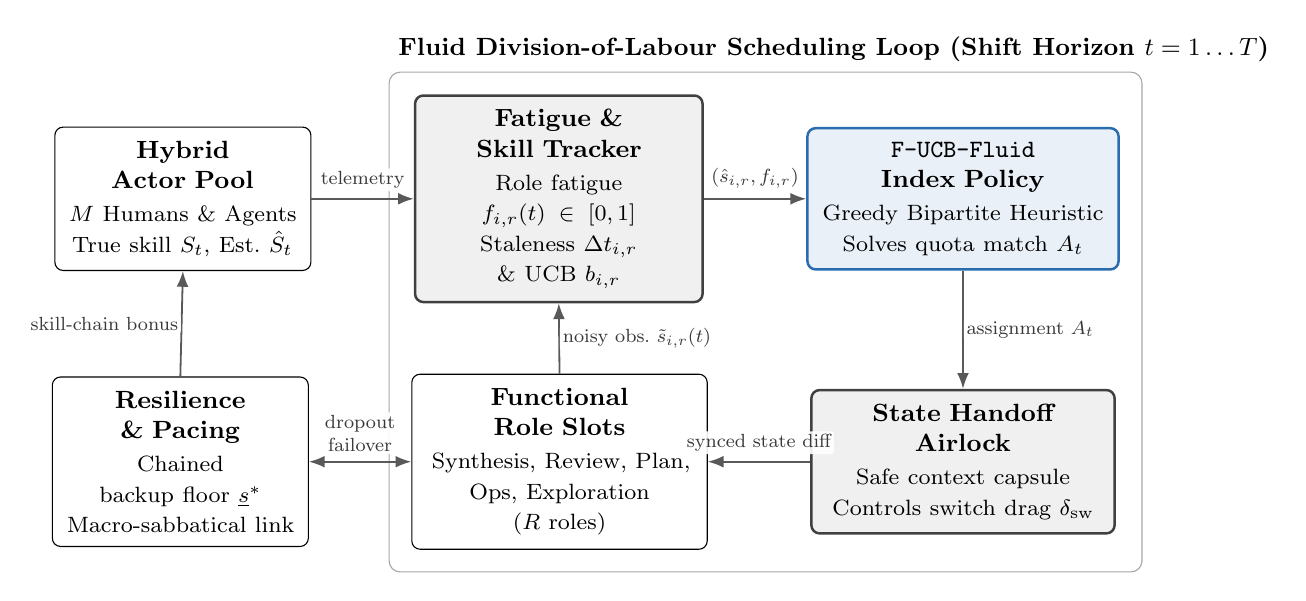
\begin{tikzpicture}[
  font=\small,
  every node/.append style={execute at begin node={\hyphenpenalty=10000\exhyphenpenalty=10000}},
  box/.style={draw, rounded corners=3pt, align=center, minimum height=1.35cm, inner sep=5pt},
  agent/.style={box, draw=accent, line width=0.9pt, fill=accent!10},
  kernel/.style={box, draw=black!75, line width=0.9pt, fill=gray!12},
  capsule/.style={draw=gray!70, rounded corners=4pt, inner sep=8pt},
  arr/.style={-{Latex[length=2mm]}, gray!70!black, line width=0.65pt},
  bidir/.style={{Latex[length=2mm]}-{Latex[length=2mm]}, gray!70!black, line width=0.65pt},
  note/.style={font=\footnotesize, scale=0.86, transform shape, text=gray!45!black, align=center, fill=white, fill opacity=0.90, text opacity=1, inner sep=1.2pt, rounded corners=1pt}
]
% ---------------- Actor Pool ----------------
\node[box, text width=2.9cm] (pool) at (0, 0) {\textbf{Hybrid Actor Pool}\\[1pt]{\footnotesize $M$ Humans \& Agents}\\{\footnotesize True skill $S_t$, Est.\ $\hat{S}_t$}};

% ---------------- Telemetry & Fatigue Estimator ----------------
\node[kernel, text width=3.3cm, right=1.3cm of pool] (state) {\textbf{Fatigue \& Skill Tracker}\\[1pt]{\footnotesize Role fatigue $f_{i,r}(t) \in [0,1]$}\\{\footnotesize Staleness $\Delta t_{i,r}$ \& UCB $b_{i,r}$}};

% ---------------- F-UCB-Fluid Bandit Scheduler ----------------
\node[agent, text width=3.6cm, right=1.3cm of state] (bandit) {\textbf{\texttt{F-UCB-Fluid} Index Policy}\\[1pt]{\footnotesize Greedy Bipartite Heuristic}\\{\footnotesize Solves quota match $A_t$}};

% ---------------- Handoff Airlock ----------------
\node[kernel, text width=3.5cm, below=1.5cm of bandit] (handoff) {\textbf{State Handoff Airlock}\\[1pt]{\footnotesize Safe context capsule}\\{\footnotesize Controls switch drag $\delta_{\mathrm{sw}}$}};

% ---------------- Active Role Slots ----------------
\node[box, text width=3.4cm, left=1.3cm of handoff] (roles) {\textbf{Functional Role Slots}\\[1pt]{\footnotesize Synthesis, Review, Plan,}\\{\footnotesize Ops, Exploration ($R$ roles)}};

% ---------------- Shock & Bus-Factor Monitor ----------------
\node[box, text width=2.9cm, left=1.3cm of roles] (monitor) {\textbf{Resilience \& Pacing}\\[1pt]{\footnotesize Chained backup floor $\underline{s}^*$}\\{\footnotesize Macro-sabbatical link}};

\draw[arr] (pool) -- node[above=2.5pt, note]{telemetry} (state);
\draw[arr] (state) -- node[above=2.5pt, note]{$(\hat{s}_{i,r}, f_{i,r})$} (bandit);
\draw[arr] (bandit) -- node[right, note]{assignment $A_t$} (handoff);
\draw[arr] (handoff) -- node[above=2.5pt, note]{synced state diff} (roles);
\draw[bidir] (monitor) -- node[above=2.5pt, note]{dropout\\failover} (roles);
\draw[arr] (roles.north) -- node[right, note]{noisy obs.\ $\tilde{s}_{i,r}(t)$} (state.south);
\draw[arr] (monitor.north) -- node[left, note]{skill-chain bonus} (pool.south);

\begin{scope}[on background layer]
\node[capsule, fit=(state)(bandit)(handoff)(roles), label={[font=\small\bfseries, anchor=south west]north west:Fluid Division-of-Labour Scheduling Loop (Shift Horizon $t = 1 \dots T$)}] (capBox) {};
\end{scope}
\end{tikzpicture}%
}
\caption{Architecture of the \texttt{F-UCB-Fluid} role-rotation framework. At each shift boundary $t$, the Fatigue and Skill Tracker updates role-specific cognitive depletion $f_{i,r}(t)$, noisy competence estimates $\hat{s}_{i,r}(t)$, and unpracticed skill decay across the $M$-actor pool. The \texttt{F-UCB-Fluid} index policy computes a quota-constrained greedy bipartite assignment $A_t$ balancing optimistic comparative-advantage yield against nonlinear fatigue barriers and chained backup skill floors.}
\label{fig:architecture}
\end{figure}

% ===============================================================
\section{Formal mathematical framework}\label{sec:formal}

We formulate fluid division of labor over discrete shift epochs $t \in \{1,\allowbreak 2,\allowbreak \dots,\allowbreak T\}$ for a cooperative collective of $M$ actors indexed by $i \in \mathcal{M} = \{1,\allowbreak \dots,\allowbreak M\}$ and $R$ functional roles indexed by $r \in \mathcal{R} = \{1,\allowbreak \dots,\allowbreak R\}$. Each role $r$ requires a quota of $q_r \in \mathbb{N}_+$ active participants per shift such that $\sum_{r=1}^R q_r \le |\mathcal{M}_t|$, where $\mathcal{M}_t \allowbreak \subseteq \mathcal{M}$ is the set of available actors at shift $t$. Let $a_{i,r}(t) \allowbreak \in \{0,\allowbreak 1\}$ denote the binary decision variable indicating whether actor $i$ is assigned to role $r$ during shift $t$, subject to $\sum_{r=1}^R a_{i,r}(t) \le 1$ for all $i \in \mathcal{M}_t$ and $\sum_{i \in \mathcal{M}_t} a_{i,r}(t) = q_r(t)$ for all $r \in \mathcal{R}$.

\subsection{Role-specific vs.\ persistent systemic fatigue and nonstationary Kalman skill tracking}

In a standard multi-armed bandit, unselected arms remain static. In human-AI work systems, however, every actor-role pair $(i, r)$ evolves continuously whether active or rested, the defining characteristic of a restless bandit \citep{whittle1988restless}. Each actor $i$ possesses a latent competence vector $\mathbf{s}_i(t) = (s_{i,1}(t),\allowbreak \dots,\allowbreak s_{i,R}(t)) \allowbreak \in [\underline{s}_{\min},\allowbreak 1]^R$, a role-specific cognitive fatigue vector $\mathbf{f}_i^{\mathrm{role}}(t) = (f_{i,1}^{\mathrm{role}}(t),\allowbreak \dots,\allowbreak f_{i,R}^{\mathrm{role}}(t)) \allowbreak \in [0,\allowbreak 1]^R$, and a persistent cross-role systemic fatigue scalar $f_i^{\mathrm{sys}}(t) \allowbreak \in [0,\allowbreak 1]$.

Grounded in the Effort-Recovery model \citep{meijman1998effort}, when actor $i$ executes role $r$ at shift $t$ ($a_{i,r}(t) = 1$), role-specific fatigue $f_{i,r}^{\mathrm{role}}(t)$ accumulates with stochastic workload intensity $\xi_{i,r}(t) \sim \mathcal{U}(0.85,\allowbreak 1.15)$ scaled by task fatigue rate $\alpha > 0$, moderated by partial between-shift overnight recovery $\gamma_{\mathrm{on}} \allowbreak \in (0,\allowbreak 1)$. When actor $i$ rotates out of role $r$ ($a_{i,r}(t) = 0$), that specific functional circuit undergoes cross-task recovery at rate $\gamma_{\mathrm{off}} < \gamma_{\mathrm{on}}$ with dissipation $\beta_{\mathrm{rest}} > 0$. Crucially, however, task rotation cannot eliminate systemic whole-worker fatigue $f_i^{\mathrm{sys}}(t)$, which accumulates across \emph{any} active shift ($\sum_{r=1}^R a_{i,r}(t) = 1$) at rate $\alpha_{\mathrm{sys}} = 0.38\alpha$ with slow overnight retention $\gamma_{\mathrm{sys}} = 0.92$, combining with role-specific fatigue via weight $\kappa_{\mathrm{sys}} \allowbreak \in [0,\allowbreak 1]$:
\begin{equation}
\begin{aligned}
f_{i,r}^{\mathrm{role}}(t+1) &\;=\; \mathbb{I}[a_{i,r}(t)=1]\min\!\bigl(1, \gamma_{\mathrm{on}} f_{i,r}^{\mathrm{role}}(t) + \alpha \xi_{i,r}(t)\bigr) \\
&\quad + \mathbb{I}[a_{i,r}(t)=0]\max\!\bigl(0, \gamma_{\mathrm{off}} f_{i,r}^{\mathrm{role}}(t) - \beta_{\mathrm{rest}}\bigr), \\
f_i^{\mathrm{sys}}(t+1) &\;=\; \min\!\Bigl(1,\; \gamma_{\mathrm{sys}} f_i^{\mathrm{sys}}(t) + \alpha_{\mathrm{sys}} \sum_{r=1}^R a_{i,r}(t)\xi_{i,r}(t)\Bigr), \\
&f_{i,r}^{\mathrm{eff}}(t) = (1 - \kappa_{\mathrm{sys}})f_{i,r}^{\mathrm{role}}(t) + \kappa_{\mathrm{sys}} f_i^{\mathrm{sys}}(t).
\end{aligned}
\label{eq:fatigue_dyn}
\end{equation}
Simultaneously, true skill competence $s_{i,r}(t)$ obeys an asymmetric learning-and-forgetting law \citep{jaber1996learning, shen2026coding, kosmyna2025brain}. Active practice increments latent competence via learning-by-doing at rate $\eta_+ = 0.0065$ per shift, whereas unpracticed roles decay at rate $\eta_- = 0.0060$ per shift toward a baseline floor $\underline{s}_{\min} = 0.35$. To establish an explicit relationship between noisy observations, nonstationary forgetting, and the uncertainty bonus, we state clearly what is observed, estimated, and forgotten:
\begin{equation}
\begin{aligned}
s_{i,r}(t+1) &\;=\; \mathbb{I}[a_{i,r}(t)=1]\min(0.99, s_{i,r}(t) + \eta_+) + \mathbb{I}[a_{i,r}(t)=0]\max(\underline{s}_{\min}, s_{i,r}(t) - \eta_-), \\
\hat{s}_{i,r}(t+1) &\;=\; \begin{cases} \min\!\bigl(0.99,\; (1 - K_{i,r}(t))\hat{s}_{i,r}(t) + K_{i,r}(t)\tilde{s}_{i,r}(t) + \hat{\eta}_+\bigr), & \text{if } a_{i,r}(t)=1, \\
\max\!\bigl(\underline{s}_{\min},\; \hat{s}_{i,r}(t) - \hat{\eta}_-\bigr), & \text{if } a_{i,r}(t)=0,
\end{cases} \\
\sigma_{i,r}^2(t+1) &\;=\; \mathbb{I}[a_{i,r}(t)=1]\bigl(1 - K_{i,r}(t)\bigr)\sigma_{i,r}^2(t) \\
&\quad + \mathbb{I}[a_{i,r}(t)=0]\min\!\bigl(0.06, \sigma_{i,r}^2(t) + \sigma_d^2\bigr),
\end{aligned}
\label{eq:skill_dyn}
\end{equation}
where only active assignments ($a_{i,r}(t)=1$) generate a noisy observation $\tilde{s}_{i,r}(t) = \mathrm{clip}(s_{i,r}(t) + \epsilon_{i,r}(t),\allowbreak 0.35,\allowbreak 0.99)$ with $\epsilon_{i,r}(t) \sim \mathcal{N}(0,\allowbreak \sigma_{\mathrm{obs}}^2)$ ($\sigma_{\mathrm{obs}} = 0.045$) and Kalman gain $K_{i,r}(t) = \sigma_{i,r}^2(t)/(\sigma_{i,r}^2(t) + \sigma_{\mathrm{obs}}^2)$, while inactive arms ($a_{i,r}(t)=0$) receive no observation and experience posterior variance inflation $\sigma_d^2 = 0.0008$ per unpracticed shift due to stochastic forgetting drift.

\subsection{Equalized nonlinear fatigue-attenuated yield and handoff drag}

To ensure a fair, non-circular comparison across all scheduling policies, the physical reward environment applies the exact same yield function and switching penalty $\delta_{\mathrm{sw}} \ge 0$ to every policy, with zero policy-specific ad-hoc drag terms. Effective productivity degrades nonlinearly with combined fatigue $f_{i,r}^{\mathrm{eff}}(t)$, and assigning an under-qualified or decayed actor ($s_{i,r}(t) < \underline{s}_{\mathrm{crit}} = 0.68$) to a role incurs a proportional quality-rework factor $\psi(s_{i,r}) = \min(1,\allowbreak \max(0.38,\allowbreak 1 - 2.2(\underline{s}_{\mathrm{crit}} - s_{i,r})))$. The realized shift output $y_{i,r}(t)$ is:
\begin{equation}
\begin{aligned}
&y_{i,r}(t) \;=\; \max\!\Bigl(y_{\min},\; s_{i,r}(t)\,\max\bigl(0.20, 1 - \kappa_f\, f_{i,r}^{\mathrm{eff}}(t)^{\nu}\bigr)\,\psi\bigl(s_{i,r}(t)\bigr) \\
&\quad \;-\; \delta_{\mathrm{sw}}\,\mathbb{I}\bigl[a_{i,r}(t-1) = 0\bigr]\Bigr),
\end{aligned}
\label{eq:shift_yield}
\end{equation}
where $\nu = 1.45$ is the nonlinear fatigue exponent, $\kappa_f = 0.82$ scales depletion severity, and $\delta_{\mathrm{sw}}$ (set to $0.072$ for all policies in the primary benchmark, and swept over $[0.012, 0.150]$ in sensitivity analysis) represents context-switching and state-reloading friction.

\subsection{The \texttt{F-UCB-Fluid} index policy: greedy vs.\ exact bipartite assignment}

Myopic greedy optimization of Equation~\eqref{eq:shift_yield} exhibits two structural blind spots: first, it exploits primary specialists until $f_{i,r}^{\mathrm{eff}}(t)^{\nu}$ enters the steep nonlinear degradation zone; second, it never invests in maintaining secondary backup skills $s_{i,r'}(t)$ above the rework threshold $\underline{s}_{\mathrm{crit}} = 0.68$, causing severe bottleneck rework if primary specialists drop out at shift $t_{\mathrm{shock}}$. \texttt{F-UCB-Fluid} addresses both by computing a composite priority index $U_{i,r}(t)$ for each candidate pair $(i, r)$:
\begin{equation}
\begin{aligned}
U_{i,r}(t) \;=\;& \underbrace{\min\!\Bigl(0.99, \hat{s}_{i,r}(t) + c_{\mathrm{ucb}}\sigma_{i,r}(t)\Bigr)\bigl(1 - \kappa_f f_{i,r}^{\mathrm{eff}}(t)^{\nu}\bigr) - \delta_{\mathrm{sw}}\mathbb{I}[r \neq r_{i,t-1}]}_{\text{Kalman-UCB Comparative-Advantage Yield}} \\
&+\; \underbrace{\omega_{i,r}\bigl(\lambda_{\mathrm{fl}}\max(0, \underline{s}^* - \hat{s}_{i,r}(t)) + \lambda_{\mathrm{st}}\max(0, \Delta t_{i,r} - 3)\bigr)(1 - f_{i,r}^{\mathrm{eff}}(t))}_{\text{Chained Backup Skill-Floor \& Staleness Bonus}} \\
&\quad \;-\; \underbrace{\lambda_{\mathrm{bar}}\max(0, f_{i,r}^{\mathrm{eff}}(t) - \theta_{\mathrm{safe}})}_{\text{Proactive Burnout Barrier}},
\end{aligned}
\label{eq:f_ucb_obj}
\end{equation}
where $c_{\mathrm{ucb}} = 1.35$ multiplies the Kalman posterior standard deviation $\sigma_{i,r}(t) = \sqrt{\sigma_{i,r}^2(t)}$, $\omega_{i,r} \allowbreak \in \{0.15,\allowbreak 0.35,\allowbreak 1.0\}$ prioritizes chained backup roles \citep{hopp2004chaining}, $\underline{s}^* = 0.75 > \underline{s}_{\mathrm{crit}}$ buffers against skill decay, $\Delta t_{i,r} = \min(16,\allowbreak t - t^{\mathrm{last}}_{i,r})$ is staleness, and $\theta_{\mathrm{safe}} = 0.42$ is the soft proactive fatigue threshold. We explicitly distinguish two assignment solvers over $U_{i,r}(t)$: (i) our fast $\mathcal{O}(MR \log(MR))$ greedy bipartite heuristic (\texttt{F-UCB-Fluid}), which assigns pairs in descending order of $U_{i,r}(t)$ subject to quotas $q_r$, and (ii) an exact dynamic-programming bipartite assignment solver (\texttt{Exact-DP-F-UCB}) that computes $A_t^* = \arg\max_{A \in \mathcal{A}_t} \sum_{i,r} a_{i,r} U_{i,r}(t)$ over the quota-state lattice.

% ===============================================================
\section{System architecture and parameter provenance}\label{sec:architecture}

To operationalize Equation~\eqref{eq:f_ucb_obj} in hybrid human-agent teams, \texttt{F-UCB-Fluid} is structured into three subsystems (Table~\ref{tab:readiness}):

\begin{enumerate}
  \item \textbf{Tier 1: Fast Bipartite Index Router and Non-Invasive Telemetry.} Role assignment decisions are decoupled from heavy LLM reasoning. A lightweight index controller evaluates Equation~\eqref{eq:f_ucb_obj} at shift boundaries in $52.5~\mu\mathrm{s}$ (greedy) or $459.8~\mu\mathrm{s}$ (exact DP), ingesting task-completion rubrics \citep{rlvr2_2026}, time-on-role counters, and optional wearable stress indicators \citep{acan2026stress, sathyanarayana2026wearables, jin2025cognitive}.
  \item \textbf{Tier 2: Safe Context-Switching Capsules.} The decisive parameter governing rotation viability is handoff friction $\delta_{\mathrm{sw}}$ \citep{das2026safecontext, rodrigues2026drift}. When an actor rotates out of a complex role, unstructured chat histories force the incoming actor to expend substantial effort reconstructing task state \citep{zhang2025agentprune}. Tier~2 requires each shift to serialize working state into a schema-validated handoff capsule (repository diff, failing assertions, and open decision variables). Rather than assuming a free handoff discount in our primary benchmark, we evaluate all policies at an equalized baseline $\delta_{\mathrm{sw}} = 0.072$ and explicitly sweep $\delta_{\mathrm{sw}} \allowbreak \in [0.012,\allowbreak 0.150]$ to quantify the return on structured state serialization.
  \item \textbf{Tier 3: Chained Backup Failover and Macro-Sabbatical Coupling.} Following skill-chaining theory \citep{hopp2004chaining} and adaptive crew topology generation \citep{li2025argdesigner, chen2026goagent}, Tier~3 ensures that critical bottleneck roles maintain cross-trained backups above $\underline{s}_{\mathrm{crit}} = 0.68$. Furthermore, because shift-to-shift cross-role recovery ($\gamma_{\mathrm{off}} = 0.52$) cannot clear persistent cross-role systemic fatigue $f_i^{\mathrm{sys}}(t)$ ($\gamma_{\mathrm{sys}} = 0.92$), Tier~3 exports cumulative systemic fatigue telemetry to a weekly-horizon sabbatical scheduler (detailed in our companion study on mandatory cooldown pacing) whenever $\kappa_{\mathrm{sys}} f_i^{\mathrm{sys}}(t)$ accumulates.
\end{enumerate}

\begin{table}[ht]
\centering
\small
\caption{Readiness and deployment bottlenecks of fluid role-rotation subsystems.}
\label{tab:readiness}
\begin{tabularx}{\textwidth}{@{}P{2.3cm}P{2.05cm}YY@{}}
\toprule
Subsystem & Maturity & Supporting empirical \& theoretical evidence & Realistic deployment bottleneck \\
\midrule
Bipartite index role router & Production ready & Restless bandit index policies \citep{whittle1988restless}; dynamic multi-agent crew assembly \citep{li2025argdesigner, zhang2025gdesigner} & Micro-rotating at sub-hour intervals inflates context-switching drag $\delta_{\mathrm{sw}}$ above break-even thresholds\\
Safe context handoff capsules & Benchmark validated & Safe context switching \citep{das2026safecontext}; context-drift synchronization \citep{rodrigues2026drift}; communication pruning \citep{zhang2025agentprune} & Tacit human intuition in open-ended design roles resists lossless compression into structured JSON diffs \\
Chained skill-floor maintenance & Theory \& field grounded & Skill-chaining in serial/parallel lines \citep{hopp2004chaining}; learning-forgetting curves \citep{jaber1996learning}; AI skill formation \citep{shen2026coding} & Over-broad cross-training across all $R$ roles dilutes specialist depth; chaining must target 1--2 backup roles\\
Cognitive fatigue \& load tracking & Field validated & Effort-Recovery model \citep{meijman1998effort}; passive stress sensing \citep{acan2026stress, jin2025cognitive}; critical thinking under load \citep{zhi2026timeconstraints} & Subjective self-assessments suffer from overconfidence \citep{eleftheriou2026confidence}; biometric sensing requires strict privacy guards \\
\bottomrule\end{tabularx}
\end{table}

\begin{table}[ht]
\centering
\small
\caption{Provenance of simulation parameters in \texttt{experiment.\linebreak[0]py}. All scheduling policies are evaluated on paired seeds with identical physical environment parameters.}
\label{tab:provenance}
\begin{tabularx}{\textwidth}{@{}P{2.2cm}P{2.1cm}P{2.5cm}Y@{}}
\toprule
Parameter & Value / Range & Provenance Type & Empirical or Theoretical Grounding \\
\midrule
Team \& horizon ($M, R, T$) & $M{=}12,\allowbreak R{=}5,\allowbreak T{=}60$ & Architectural design & Typical squad size and 60-shift (12-week) project horizon in hybrid software/ops collectives \citep{cemri2025mast, kim2025scaling}\\
Initial competence $s_{i,r}(0)$ & Primary $[0.88,0.96]$, Backup $[0.72,0.80]$ & Calibrated prior & Tiered specialist, chained backup, and generalist proficiency hierarchy \citep{hopp2004chaining, ortega2001jobrotation}\\
Learning \& decay $(\eta_+,\allowbreak \eta_-)$ & $+0.0065,\allowbreak -0.0060$ per shift & Literature-calibrated & Asymmetric learning-and-forgetting curves and Kalman variance drift $\sigma_d^2 = 0.0008$ \citep{jaber1996learning, shen2026coding}\\
Role \& systemic fatigue $(\gamma_{\mathrm{on}},\allowbreak \gamma_{\mathrm{off}},\allowbreak \kappa_{\mathrm{sys}})$ & $\gamma_{\mathrm{on}}{=}0.84,\allowbreak \gamma_{\mathrm{off}}{=}0.52$, $\kappa_{\mathrm{sys}} \allowbreak \in [0,\allowbreak 0.90]$ & Parameterized sweep & Effort-Recovery dynamics \citep{meijman1998effort} separating cross-task recovery from persistent systemic fatigue\\
Nonlinear fatigue $(\kappa_f,\allowbreak \nu)$ & $\kappa_f{=}0.82,\allowbreak \nu{=}1.45$ & Stylized functional form & Convex productivity attenuation under accumulated cognitive load \citep{zhi2026timeconstraints, acan2026stress}\\
Switch penalty $\delta_{\mathrm{sw}}$ & $0.072$ (swept $0.012\text{--}0.150$) & Equalized benchmark + sensitivity sweep & Context-reload overhead \citep{das2026safecontext, zhang2025agentprune} held strictly equal across all policies in primary runs\\
\bottomrule\end{tabularx}
\end{table}

% ===============================================================
\section{Simulation evaluation and sensitivity analysis}\label{sec:experiments}

We evaluate \texttt{F-UCB-Fluid} using a paired Monte Carlo simulation suite (\texttt{experiment.\linebreak[0]py}): $N=500$ paired sixty-shift episodes across four greedy policies and four fatigue rates $\alpha \in \{0.10,\allowbreak 0.16,\allowbreak 0.22,\allowbreak 0.28\}$ ($8{,}000$ main trajectories), a $400$-episode small-instance optimality benchmark comparing greedy \texttt{F-UCB-Fluid} against exact dynamic-programming assignment (\texttt{Exact-DP-F-UCB}), $4{,}500$ sensitivity trajectories across $\delta_{\mathrm{sw}} \allowbreak \in \{0.012,\allowbreak 0.024,\allowbreak 0.048,\allowbreak 0.072,\allowbreak 0.110,\allowbreak 0.150\}$, and $2{,}500$ trajectories across persistent systemic fatigue weight $\kappa_{\mathrm{sys}} \allowbreak \in \{0.00,\allowbreak 0.20,\allowbreak 0.45,\allowbreak 0.70,\allowbreak 0.90\}$.

\subsection{Equally tuned baseline schedulers and specialist dropout protocol}

To test bus-factor resilience without artificial handicaps, during shifts $t \in [40, 49]$ two of the three primary Role-0 specialists (actors $0$ and $5$) go offline while Role~0 still requires $q_0 = 3$ active operators, forcing at least two non-primary actors to cover Role~0. If those backups allowed their Role-0 competence to decay below $\underline{s}_{\mathrm{crit}} = 0.68$, Equation~\eqref{eq:shift_yield} applies the rework penalty $\psi(s_{i,0})$. All policies operate on identical paired episode seeds (\texttt{ep\_\linebreak[0]seed = 20261143 + 97 * ep\_\linebreak[0]idx}) under $\delta_{\mathrm{sw}} = 0.072$ and $\kappa_{\mathrm{sys}} = 0.20$:
\begin{itemize}
  \item \textbf{Specialist + Rest-Swap (\texttt{specialist\_\linebreak[0]rest}):} Tuned with the exact same proactive fatigue threshold $\theta_{\mathrm{safe}} = 0.42$ as \texttt{F-UCB-Fluid}; prioritizes each actor's primary role when $f_{i,r}^{\mathrm{eff}}(t) < 0.42$, grants a restorative rotation into a low-fatigue secondary role whenever primary fatigue exceeds $0.42$, and re-optimizes over available actors during the $t \in [40, 49]$ dropout shock.
  \item \textbf{Periodic Round-Robin Rotation (\texttt{blind\_\linebreak[0]rotation}):} Rotates all actors across roles every 4 shifts on a fixed clock, with zero ad-hoc mismatch penalty beyond Equation~\eqref{eq:shift_yield}.
  \item \textbf{Myopic Greedy / Whittle Heuristic (\texttt{whittle\_\linebreak[0]greedy}):} Assigns pairs at each shift to maximize instantaneous fatigue-attenuated yield minus switch cost ($\hat{s}_{i,r}(t)(1 - \kappa_f f_{i,r}^{\mathrm{eff}}(t)^{\nu}) - \delta_{\mathrm{sw}}\mathbb{I}[r \neq r_{i,t-1}]$), without Kalman-UCB exploration or backup skill-floor regularization.
  \item \textbf{Fatigue-Aware UCB Index Policy (\texttt{f\_\linebreak[0]ucb\_\linebreak[0]fluid} / \texttt{Exact-DP-F-UCB}, Proposed):} Evaluates Equation~\eqref{eq:f_ucb_obj} via either the fast greedy bipartite solver (\texttt{f\_\linebreak[0]ucb\_\linebreak[0]fluid}) or the exact dynamic-programming bipartite assignment solver (\texttt{Exact-DP-F-UCB}).
\end{itemize}

\begin{table}[ht]
\centering
\small
\caption{Paired benchmark across simulated 60-shift workflows ($\alpha=0.22$, $\delta_{\mathrm{sw}} = 0.072$, $\kappa_{\mathrm{sys}} = 0.20$; $N=500$ episodes per greedy policy and $N=200$ episodes for \texttt{Exact-DP-F-UCB}). All intervals report asymmetric 95\% confidence bounds $[\mathrm{lo},\allowbreak \mathrm{hi}]$ (continuous SEM bounds for yield/resilience and exact two-sided Wilson score bounds for binary shock survival $\ge 72\%$).}
\label{tab:results}
{\footnotesize\setlength{\tabcolsep}{3.0pt}%
\begin{tabularx}{\textwidth}{@{}P{2.35cm}RRRRRr@{}}
\toprule
Scheduler Policy & Yield $\alpha{=}0.10$ (\%) & Yield $\alpha{=}0.22$ (\%) & Yield $\alpha{=}0.28$ (\%) & Bus-Factor Resil.\ (\%) & Shock Survival (\%) & \shortstack[r]{Runtime\\($\mu$s)}\\
\midrule
Specialist + Rest-Swap & 74.02 {\scriptsize [73.97,\allowbreak 74.06]} & 68.92 {\scriptsize [68.85,\allowbreak 69.00]} & 67.29 {\scriptsize [67.24,\allowbreak 67.35]} & 69.30 {\scriptsize [69.15,\allowbreak 69.44]} & 7.60 {\scriptsize [5.59,\allowbreak 10.26]} & 14.9\\
Periodic Rotation & 60.79 {\scriptsize [60.73,\allowbreak 60.86]} & 48.41 {\scriptsize [48.36,\allowbreak 48.46]} & 43.78 {\scriptsize [43.73,\allowbreak 43.82]} & 57.49 {\scriptsize [57.44,\allowbreak 57.55]} & 0.00 {\scriptsize [0.00,\allowbreak 0.76]} & 15.1\\
Myopic Greedy Index & 76.84 {\scriptsize [76.78,\allowbreak 76.91]} & 70.57 {\scriptsize [70.49,\allowbreak 70.64]} & 68.91 {\scriptsize [68.84,\allowbreak 68.97]} & 71.06 {\scriptsize [70.94,\allowbreak 71.18]} & 24.40 {\scriptsize [20.84,\allowbreak 28.35]} & 19.9\\
\textbf{\texttt{F-UCB-Fluid} (Greedy)} & \textbf{83.15} {\scriptsize \textbf{[83.11,\allowbreak 83.19]}} & \textbf{73.16} {\scriptsize \textbf{[73.10,\allowbreak 73.21]}} & \textbf{70.65} {\scriptsize \textbf{[70.59,\allowbreak 70.70]}} & \textbf{74.79} {\scriptsize \textbf{[74.69,\allowbreak 74.89]}} & \textbf{99.00} {\scriptsize \textbf{[97.68,\allowbreak 99.57]}} & \textbf{52.5}\\
\textbf{\texttt{Exact-DP-F-UCB}} & --- & \textbf{74.73} {\scriptsize \textbf{[74.64,\allowbreak 74.82]}} & --- & \textbf{76.61} {\scriptsize \textbf{[76.47,\allowbreak 76.74]}} & \textbf{100.00} {\scriptsize \textbf{[98.12,\allowbreak 100.00]}} & \textbf{459.8}\\
\bottomrule\end{tabularx}}
\end{table}

\subsection{Quantitative findings: exact DP gap, handoff drag, and systemic fatigue}

Table~\ref{tab:results} and Figures~\ref{fig:benchmark}--\ref{fig:ablation} establish four empirical findings:
\begin{enumerate}
  \item \textbf{Superiority over equally tuned rest-swaps and myopic greedy indexing.} Even when \texttt{specialist\_\linebreak[0]rest} is tuned with the exact same proactive rest-swap threshold ($\theta_{\mathrm{safe}} = 0.42$), its secondary Role-0 backups experience unpracticed skill decay below $\underline{s}_{\mathrm{crit}} = 0.68$ prior to shift~$40$, resulting in $69.30\%$ [$69.15, 69.44$] bus-factor resilience and only $7.60\%$ [$5.59, 10.26$] ($38/500$) shock survival at $\alpha=0.22$. Myopic Greedy Index (\texttt{whittle\_\linebreak[0]greedy}) reaches $70.57\%$ [$70.49, 70.64$] yield and $24.40\%$ [$20.84, 28.35$] ($122/500$) shock survival. By combining Kalman-UCB competence tracking ($\sigma_{i,r}(t)$) with chained backup skill-floor maintenance, greedy \texttt{F-UCB-Fluid} achieves $73.16\%$ [$73.10, 73.21$] net yield, $74.79\%$ [$74.69, 74.89$] bus-factor resilience, and $99.00\%$ [$97.68, 99.57$] ($495/500$) shock survival while maintaining $98.92\%$ burnout-free shifts.
  \item \textbf{Greedy heuristic vs.\ exact dynamic-programming bipartite optimum.} Comparing greedy \texttt{F-UCB-Fluid} against exact combinatorial assignment (\texttt{Exact-DP-F-UCB}) across $N=200$ paired episodes at $\alpha=0.22$ shows that the greedy bipartite solver achieves $98.62\%$ of the exact single-step DP index sum on average, yielding $73.15\%$ [$73.07, 73.24$] vs.\ $74.73\%$ [$74.64, 74.82$] trajectory yield while reducing per-shift solver latency by $8.8\times$ ($52.5~\mu\mathrm{s}$ vs.\ $459.8~\mu\mathrm{s}$).
  \item \textbf{Handoff-penalty sensitivity and break-even regime.} Sweeping $\delta_{\mathrm{sw}} \allowbreak \in \{0.012,\allowbreak 0.024,\allowbreak 0.048,\allowbreak 0.072,\allowbreak 0.110,\allowbreak 0.150\}$ at $\alpha=0.22$ confirms that structured handoff capsules \citep{das2026safecontext} strongly amplify rotation gains: at $\delta_{\mathrm{sw}} = 0.024$ ($\delta_{\mathrm{sw}} = 0.012$), \texttt{F-UCB-Fluid} yield rises to $78.02\%$ [$77.94, 78.10$] ($79.34\%$ [$79.26, 79.43$]) with $80.41\%$ ($81.97\%$) bus-factor resilience. Conversely, at $\delta_{\mathrm{sw}} = 0.150$, yield compresses to $69.07\%$ [$68.96, 69.17$].
  \item \textbf{Persistent cross-role systemic fatigue ($\kappa_{\mathrm{sys}}$) and necessity of macro-sabbicals.} Sweeping the systemic fatigue coupling weight $\kappa_{\mathrm{sys}} \allowbreak \in \{0.00,\allowbreak 0.20,\allowbreak 0.45,\allowbreak 0.70,\allowbreak 0.90\}$ demonstrates a critical ergonomic boundary: when fatigue is purely or predominantly role-specific ($\kappa_{\mathrm{sys}} = 0.00$ and $0.20$), \texttt{F-UCB-Fluid} achieves $78.49\%$ and $73.14\%$ net yield with $99.17\%$ and $98.92\%$ burnout-free shifts. However, when persistent cross-role exhaustion dominates ($\kappa_{\mathrm{sys}} = 0.45,\allowbreak 0.70,\allowbreak 0.90$), net yield falls to $62.39\%$, $49.03\%$, and $40.54\%$, and burnout-free shifts drop to $96.25\%$, $44.06\%$, and $26.92\%$. Because role rotation cannot clear systemic fatigue $f_i^{\mathrm{sys}}(t)$, high-$\kappa_{\mathrm{sys}}$ regimes require coupling shift-level rotation with periodic multi-week sabbatical cooldowns.
\end{enumerate}

\begin{figure}[ht]
\centering
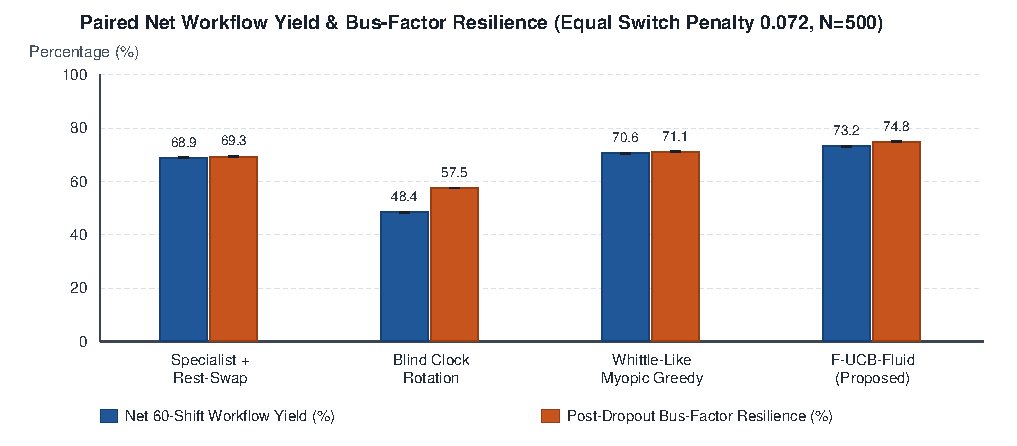
\includegraphics[width=0.88\textwidth]{figures/fig1_benchmark.pdf}
\caption{Paired comparison of Net Cooperative Yield and Specialist-Dropout Bus-Factor Resilience across four schedulers at $\alpha=0.22$, $\delta_{\mathrm{sw}}=0.072$, and $\kappa_{\mathrm{sys}}=0.20$ ($N=500$ episodes per policy; error bars denote 95\% confidence intervals).}
\label{fig:benchmark}
\end{figure}

\begin{figure}[ht]
\centering
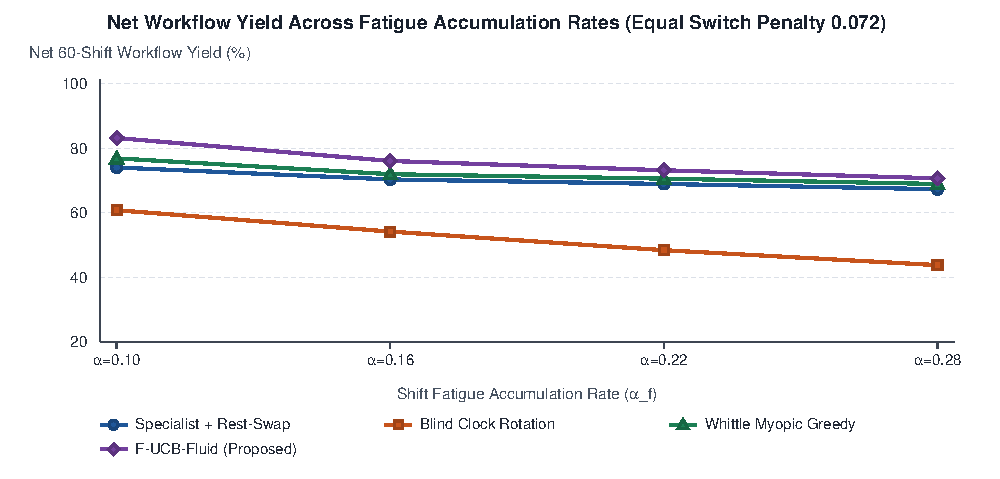
\includegraphics[width=0.86\textwidth]{figures/fig2_ablation.pdf}
\caption{Scaling of Net Cooperative Yield across shift cognitive fatigue rates $\alpha \in \{0.10,\allowbreak 0.16,\allowbreak 0.22,\allowbreak 0.28\}$ under equalized switching penalty $\delta_{\mathrm{sw}}=0.072$ and systemic fatigue weight $\kappa_{\mathrm{sys}}=0.20$.}
\label{fig:ablation}
\end{figure}

% ===============================================================
\section{Operational boundary conditions and failure modes}\label{sec:counter}

We highlight four empirical boundary conditions from operations research and 2025--2026 human-AI literature where fluid division of labor can degrade collective performance:

\begin{enumerate}
  \item \textbf{Communication overhead and context drift under frequent handoffs (\citet{zhang2025agentprune, rodrigues2026drift, bertalanic2026consensus}).} \citet{zhang2025agentprune} and \citet{bertalanic2026consensus} show that inter-agent state synchronization can consume substantial token budgets and propagate correlated errors when shared context is noisy, while \citet{rodrigues2026drift} demonstrate that unsynchronized handoffs induce context drift. As confirmed by our sensitivity sweep, if $\delta_{\mathrm{sw}} \ge 0.150$, frequent rotation erodes comparative-advantage surplus.
  \item \textbf{Overconfidence and miscalibrated skill priors (\citet{eleftheriou2026confidence, vaccaro2024combinations}).} In meta-analyses of human-AI combinations, \citet{vaccaro2024combinations} find that human-AI teams frequently underperform the better of the human or AI alone on decision tasks when task allocation is miscalibrated, and \citet{eleftheriou2026confidence} document systematic overconfidence among AI-assisted knowledge workers. If competence estimates $\hat{s}_{i,r}(t)$ rely on subjective confidence rather than objective verification rubrics \citep{rlvr2_2026}, \texttt{F-UCB-Fluid} will rotate under-qualified actors into critical bottleneck roles.
  \item \textbf{Unsafe context carryover across security boundaries (\citet{das2026safecontext}).} \citet{das2026safecontext} prove that when agents switch operational contexts without strict memory sanitization, residual instructions or permissive priors from an exploratory role can compromise downstream safety-critical execution.
  \item \textbf{Irreducible credential and regulatory boundaries.} In high-hazard physical or legally licensed professions, regulatory accountability prohibits rotating uncredentialed generalists into specialist slots. In such environments, skill chaining \citep{hopp2004chaining} must be restricted strictly within certified equivalence classes.
\end{enumerate}

% ===============================================================
\section{Limitations}\label{sec:limits}

\begin{itemize}
  \item \textbf{Stylized parametric simulation.} While our learning, forgetting, and effort-recovery parameters are grounded in qualitative laws from operations research \citep{jaber1996learning, hopp2004chaining, meijman1998effort}, the numerical values in Table~\ref{tab:provenance} represent a calibrated mechanistic model rather than econometric fits to a specific live organization.
  \item \textbf{Single-step bipartite optimization vs.\ multi-step restless DP.} While we benchmark our greedy $\mathcal{O}(MR\log(MR))$ solver against exact single-step dynamic programming (\texttt{Exact-DP-F-UCB}, $98.62\%$ per-shift ratio), neither solver computes the PSPACE-hard multi-step lookahead policy over the full horizon $T$.
  \item \textbf{Inability of task rotation to clear systemic fatigue ($\kappa_{\mathrm{sys}} \ge 0.45$).} As shown in our $\kappa_{\mathrm{sys}}$ sweep, shift-level rotation only relieves role-specific depletion $f_{i,r}^{\mathrm{role}}(t)$; persistent cross-role exhaustion $f_i^{\mathrm{sys}}(t)$ requires coupling \texttt{F-UCB-Fluid} with macro-horizon mandatory sabbatical cooldowns.
\end{itemize}

% ===============================================================
\section{Pre-registerable falsification protocol}\label{sec:protocol}

Table~\ref{tab:protocol} defines six pre-registerable empirical protocols designed to falsify the core claims of \texttt{F-UCB-Fluid}.

\begin{table}[ht]
\centering
\small
\caption{Six pre-registerable empirical tests that could falsify the \texttt{F-UCB-Fluid} framework.}
\label{tab:protocol}
\begin{tabularx}{\textwidth}{@{}P{2.3cm}YYY@{}}
\toprule
Protocol & Hypothesis & Design and primary metrics & Falsified if \\
\midrule
P1. Multi-agent deadlock recovery & Rotating Reviewer and Implementer roles breaks verification deadlocks \citep{cemri2025mast, lai2026clasharness} & Benchmark 5-agent crews on 200 long-horizon SWE-bench tasks comparing Static Roles vs.\ \texttt{F-UCB-Fluid} & \texttt{F-UCB-Fluid} fails to improve task resolution rate by $\ge 5$ percentage points over static role assignment\\
P2. Handoff capsule drag reduction ($\delta_{\mathrm{sw}}$) & Safe context-switching capsules \citep{das2026safecontext} reduce post-rotation orientation overhead & Measure token usage and first-turn error rates across 400 role switches with vs.\ without schema-validated handoff capsules & Structured capsules reduce post-handoff orientation tokens or errors by $<25\%$ relative to raw transcript handoffs\\
P3. Human cognitive fatigue \& stress & Proactive rotation at $\theta_{\mathrm{safe}}=0.42$ lowers developer stress without reducing output quality & 6-week crossover trial with 48 software engineers rotating across Feature Dev, Code Review, and Triage \citep{acan2026stress, zhi2026timeconstraints} & Passive physiological stress or NASA-TLX fatigue shows no statistically significant reduction ($p \ge 0.05$)\\
P4. Chained backup skill retention & Staleness-regularized chaining prevents AI-induced skill decay \citep{jaber1996learning, shen2026coding} & Unassisted post-trial domain assessments in each participant's chained backup role after 60 shifts & Mean unassisted backup-role score falls below the rework threshold $\underline{s}_{\mathrm{crit}} = 0.68$\\
P5. Specialist dropout bus-factor shock & Skill-chained teams sustain $\ge 72\%$ throughput when two primary specialists drop out & Inject unannounced 10-shift specialist removal at $t=40$ across 200 hybrid team trajectories & Post-shock throughput under \texttt{F-UCB-Fluid} fails to exceed Specialist + Rest-Swap by $\ge 4$ percentage points\\
P6. Context sanitization on role switch & Context-reset guards \citep{das2026safecontext, rodrigues2026drift} prevent persona bleed across shifts & Audit 1{,}000 post-rotation agent turns for role-boundary violations after switching from Exploration to Verification & Post-switch boundary violation rate exceeds $2.5\%$\\
\bottomrule\end{tabularx}
\end{table}

% ===============================================================
\section{Conclusion}\label{sec:conclusion}

Neither rigid specialization nor blind periodic rotation provides a viable foundation for long-horizon human-AI collectives. By formulating division of labor as a constrained restless bandit with nonstationary Kalman competence estimation and two-component role/systemic fatigue dynamics \citep{whittle1988restless, jaber1996learning}, we show on paired simulations ($\alpha=0.22,\allowbreak \delta_{\mathrm{sw}} = 0.072,\allowbreak \kappa_{\mathrm{sys}} = 0.20$) that \texttt{F-UCB-Fluid} achieves $73.16\%$ [$73.10, 73.21$] net cooperative yield, $74.79\%$ [$74.69, 74.89$] bus-factor resilience, and $99.00\%$ [$97.68, 99.57$] shock survival, capturing $98.62\%$ of the single-step exact dynamic-programming optimum (\texttt{Exact-DP-F-UCB}, $74.73\%$ yield) at $8.8\times$ lower latency while delineating the exact handoff-drag ($\delta_{\mathrm{sw}} \ge 0.150$) and systemic-fatigue ($\kappa_{\mathrm{sys}} \ge 0.45$) boundaries where rotation must be paired with structured context capsules and macro-sabbatical cooldowns.

% ===============================================================
\section*{Use of AI tools}
Large language models were used to assist in drafting prose, formatting \LaTeX{} tables and TikZ diagrams, and implementing the standalone Python simulation script (\texttt{experiment.\linebreak[0]py}). Cited references were assembled from foundational computer-science literature and 2024--2026 research publications and checked against primary metadata records; simulation outputs, confidence intervals, and \LaTeX{} source packaging were verified using automated static consistency checks (\texttt{validate\_\linebreak[0]and\_\linebreak[0]package.\linebreak[0]py}).

\bibliographystyle{plainnat}
\bibliography{references}

\end{document}
